% 2005 年全国卷Ⅰ文科第 4 题：多面体 ABCDEF
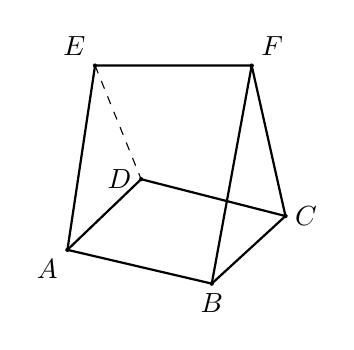
\begin{tikzpicture}[>=stealth,scale=0.78]
  \coordinate (A) at (0,0); \coordinate (B) at (2.35,-0.55);
  \coordinate (C) at (3.55,0.55); \coordinate (D) at (1.2,1.15);
  \coordinate (E) at (0.45,3.0); \coordinate (F) at (3.0,3.0);
  \draw[thick] (A)--(B)--(C)--(D)--cycle;
  \draw[thick] (A)--(E)--(F)--(B);
  \draw[thick] (C)--(F);
  \draw[dashed] (E)--(D) (D)--(C);
  \fill (A) circle (1pt) node[below left] {$A$};
  \fill (B) circle (1pt) node[below] {$B$};
  \fill (C) circle (1pt) node[right] {$C$};
  \fill (D) circle (1pt) node[left] {$D$};
  \fill (E) circle (1pt) node[above left] {$E$};
  \fill (F) circle (1pt) node[above right] {$F$};
\end{tikzpicture}
